%%
% TUM Corporate Design LaTeX Templates
% Based on the templates from https://www.tum.de/cd
%
% Feel free to join development on
% https://gitlab.lrz.de/tum-templates/templates
% and/or to create an issue in case of trouble.
%
% tum-book class for lecture notes, Master's/Bachelor's thesis, ...
%
%%

\documentclass[oneside]{tum-book}

\title{Research Internship with RCS@TUM}
\subtitle{Implementation of tiny machine learning models on microcontrollers}
\author{Philipp van Kempen}
\publisher{Chair of Real-Time Computer Systems\\
  Department of Electrical and Computer Engineering}
%\titledescription{Wissenschaftliche Arbeit zur Erlangung des Grades\\
%  \textbf{Master of Science}\\
%  an der Fakultät für Elektrotechnik und Informationstechnik der Technischen
%  Universität München.}
\titledescription{Research Internship Report\\
  \textbf{24.08.2020 - 25.10.2020}\\
  }
\fineprint{%
  \textbf{Supervised by}\\
  M.E, M.Sc Alex Hoffman\\
  Chair of Real-Time Computer Systems\\
  \vspace{12pt}
  \textbf{Author}\\
  Philipp van Kempen\\
  Sepp-Manger-Str. 3b\\
  85375 Neufahrn b. Freising\\
  \vspace{12pt}
  \textbf{Submitted}\\
  03.12.2020
}

%\usepackage[intoc,prefix]{nomencl}
%\makenomenclature

%%% NEW

\usepackage{multirow}
%\usepackage[table]{xcolor}
\usepackage[utf8]{inputenc}
\usepackage{multirow}
\usepackage{hhline}
\usepackage{colortbl}
\usepackage{multicol}
\usepackage{caption}
\usepackage{subcaption}
\usepackage{hyperref}

\definecolor{myblue}{HTML}{3366CC}
\definecolor{myblue2}{HTML}{99CCFF}
\definecolor{myblue3}{HTML}{6699FF}
\definecolor{myblue4}{HTML}{3366FF}
\definecolor{myorange}{HTML}{FF6633}
\definecolor{myorange2}{HTML}{FFCCCC}
\definecolor{myorange3}{HTML}{FFCC99}
\definecolor{myorange4}{HTML}{FF9966}
\definecolor{mygreen}{HTML}{669933}
\definecolor{mygreen2}{HTML}{CCFFCC}
\definecolor{mygreen3}{HTML}{99CC99}
\definecolor{mygreen4}{HTML}{669966}
\definecolor{myyellow}{HTML}{FFCC00}
\definecolor{myyellow2}{HTML}{FFFFCC}
\definecolor{myyellow3}{HTML}{FFCC66}
\definecolor{myyellow4}{HTML}{FFCC33}
\definecolor{mygray}{HTML}{333333}
\definecolor{mygray2}{HTML}{CCCCCC}
\definecolor{mygray3}{HTML}{999999}
\definecolor{mygray4}{HTML}{666666}


\begin{document}

%\printthesisdisclaimer{München, 29.04.2016}{Honest Student}

%\printdedication{Dedicated to Franz X. Gabelsberger, inventor of the street
%  named after him.}

\frontmatter

%\chapter{Abstract}

%My abstract goes here.

%\cleardoublepage
%\printnomenclature[3cm]

%\nomenclature{$\rho_{phen}$}{Phenomenological term that represents scattering processes in the active region}
%\nomenclature{$\hbar$}{Reduced Planck constant}

%\tableofcontents

\mainmatter

\chapter{Introduction}
\vspace{-1em}
Neural networks and artificial intelligence are omnipresent topics in today's society and economy. Examples can be found as computer vision implementations for the automotive industry and spam detection filters used by email providers.
\vspace{-1em}
\section{Motivation}

Machine Learning focuses on the development of data-dependent computer programs which are able to adapt themselves according to an optimization problem. While just a few decades ago only a small subset of electronic devices was able to run those compute-intensive algorithms, they became more and more relevant for data centers, personal computers and lastly portable devices like smartphones from time to time. Currently the exploitation of artificial models on edge devices like microcontrollers with memory capacities as low as just a couple of 100 kilobytes is a huge research topic. This trend can be also seen in the Gartner Hype Cycles, which are a graphical depiction of a common pattern that arises with each new technology or other innovation. In the release for 2020, shown in figure \ref{fig:gartner2020}, AI-related topics and especially 'Embedded AI' are dominating the field of technologies.

\begin{figure}[h]
\centering
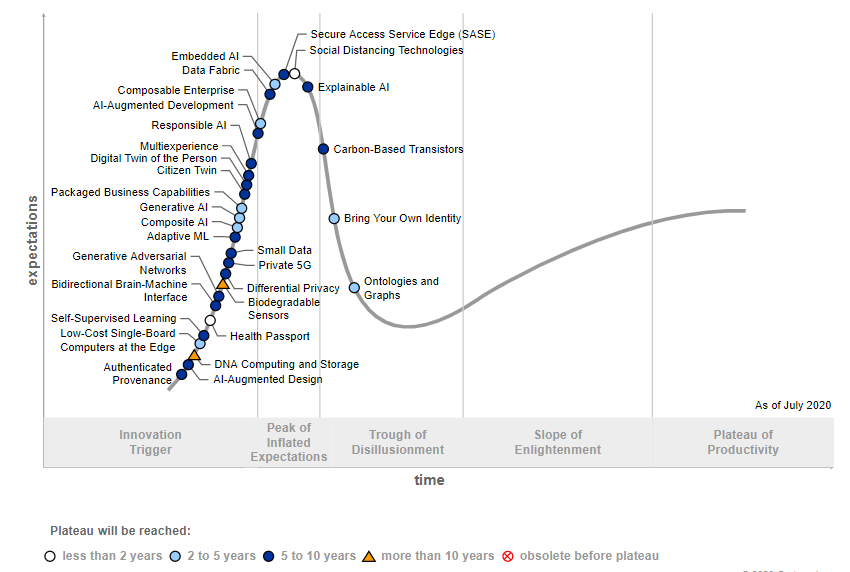
\includegraphics[width=0.75\textwidth]{figures/2020_08_23_medialist_gartner_hype_cycle_2020.png}
\caption{Gartner Hype Cycle for 2020 \cite{2020hypecycles}}
\label{fig:gartner2020}
\end{figure}

\section{Goals}

In the 9 weeks long research internship at the research group for Electronic System Level (ESL) applications founded by the chair of Electronic Design Automation (EDA) and the chair of Real-time Computer Systems (RCS), reference implementations for running TinyML\footnote{https://www.tinyml.org/summit/}-Models on STM32 Evaluation Boards had to be designed. While an initial open-source toolchain for the project already existed, it had to be extended with essential features and extensive documentation.

\chapter{Steps}

About a third of the time during the research internship was spent studying literature on the topic. The TinyML book \cite{warden2020tinyml} was the most helpful but web research was also omnipresent.

Before getting the actual examples running, the outdated toolchain had to be modified as it was written for comparatively old versions of Tensorflow. To make this step a little bit easier, the official ARM Mbed \footnote{\url{https://os.mbed.com}} was regularly used as an reference.

Another important part of the process was understanding the provided training scripts. This also involved running slightly modified versions of those scripts to tune the resulting accuracy and model sizes.

The implementation of the hello\_world example was trivial as it wokrd out of the box on the STM32 Hardware. The more complex micro\_speech demo was not working at all. While mnist had similar problems it was done way faster because the findings of the previous step. Time was mostly spent for improving the usability by adding special features.

The last essential part of the project was writing the documentation. With the help of another student, it was done in approximately 3 weeks at the end of the FP period.

The time needed for completing the tasks over the duration of the internship is depicted in figure \ref{fig:schedule}.

\begin{figure}[h]
\centering
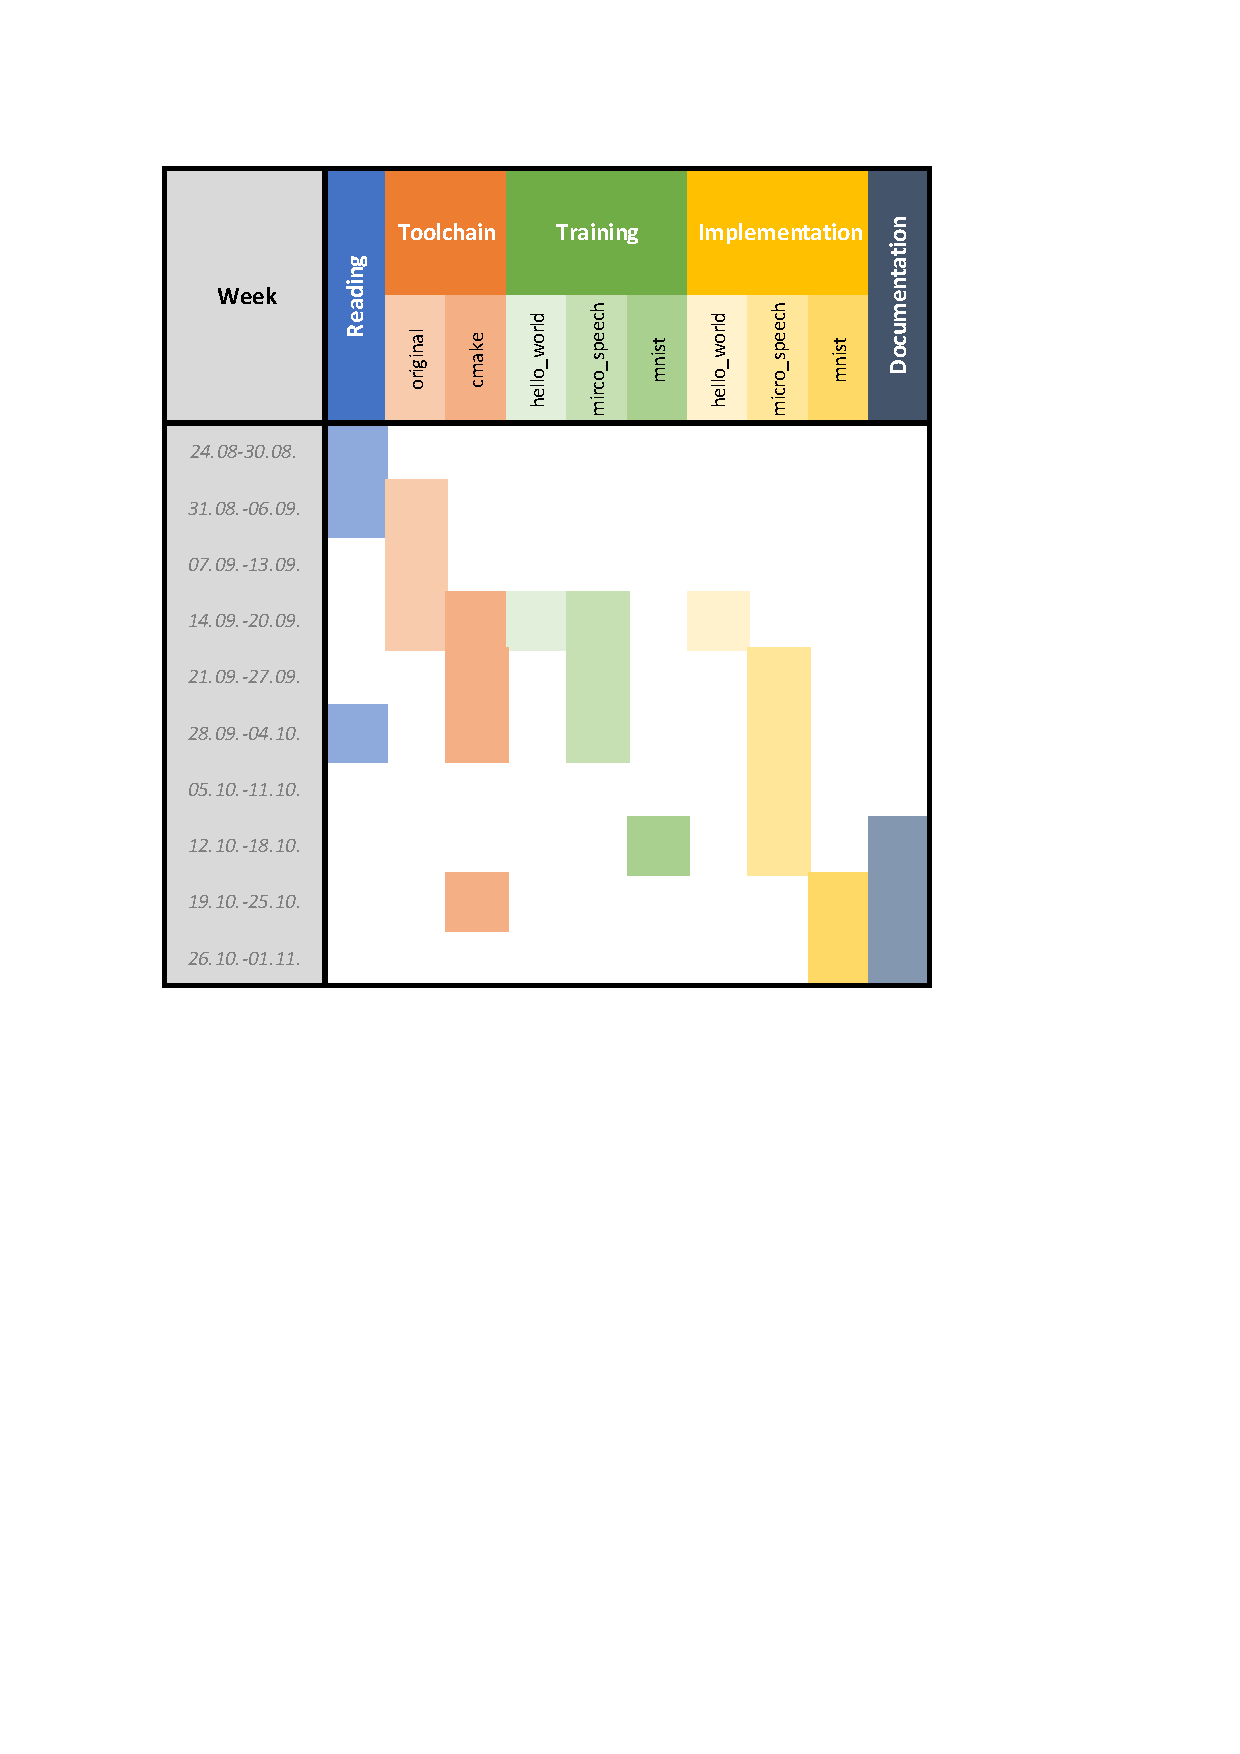
\includegraphics[scale=0.9]{figures/fp_report_plan.pdf}
\caption{Schedule}
\label{fig:schedule}
\end{figure}

\section{Reading}

The book by Pete Warden and Daniel Situnayake introduces the usage of the Tensorflow Lite for Microcontrollers (TFLM) framework in a very detailed way. Two of the practical applications, which are all referencing examples located in the Tensorflow source tree, are especially interesting as they are supported a a large number of platforms:

\begin{itemize}
    \item \textbf{Hello World:} A very simple model designed to approximate the value in the trigonometric sine function for a given x-value. As the memory and performance requirements for running this program are very low, it is often used to teach the basics of machine learning.
    \item \textbf{Micro Speech:} Inspired by voice assistants found in devices like smartphones, TVs,... which are able to detect full sentences of human speech via a microphone, this model can classify the voice commands 'yes' and 'no'. Those models, which can only detect single words are often referred as Keyword-Spotting (KWS) models. Running those models on low-power MCUs in embedded devices allows to wake up a larger processor if certain commands are detected as there accuracy alone is often not good enough for reliable results. 
\end{itemize}

In addition to the book, the official documentation of Tensorflow was a great resource to git started with the topic. It was especially helpful as it contains information for old the latest versions 2.3 of the framework as well as for Tensorflow 1.5 which is still used often in many older models.

\section{Toolchain}

The target devices for the implementations are STM32 Evaluation Boards like the following:

\begin{figure}[h]
     \centering
     \begin{subfigure}[b]{0.4\textwidth}
         \centering
         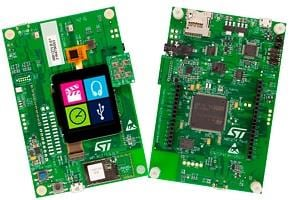
\includegraphics[width=0.6\textwidth]{figures/disco_f413h.jpg}
         \caption{STM32F413H-DISCOVERY\footnote{\url{https://www.st.com/en/evaluation-tools/32f413hdiscovery.html}}}
         \label{fig:stm32f4}
     \end{subfigure}
     \hfill
     \begin{subfigure}[b]{0.4\textwidth}
         \centering
         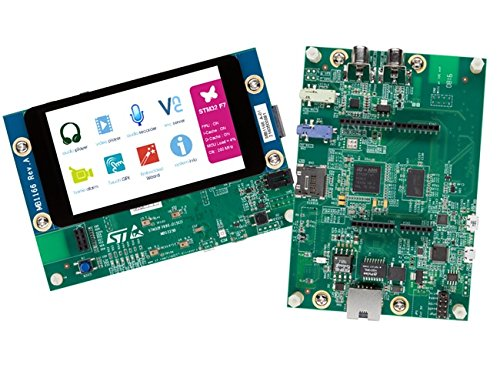
\includegraphics[width=0.6\textwidth]{figures/disco_f769i.jpg}
         \caption{STM32F769I-DISCOVERY\footnote[2]{\url{https://www.st.com/en/evaluation-tools/32f769idiscovery.html}}}
         \label{fig:stm32f7}
     \end{subfigure}
        \caption{Target Boards}
        \label{fig:boards}
\end{figure}

The CMake-based toolchain for those boards was initially developed by Konstantin Oblaukhov \footnote{\url{https://github.com/ObKo/stm32-cmake}} and further improved by Alex Hoffman in a reference application \footnote{\url{https://github.com/alxhoff/STM3240G-EVAL-TensorFlow-MNIST}}.

First, the CMake Modules had to be patched to support the components on the mentioned boards (LCD, Touchscreen, Microphone,...). With the example demonstrations from the official manufacturer firmware \footnote{\url{https://github.com/STMicroelectronics/STM32CubeF7}} it was possible to create demo applications making use of these peripherals.

To integrate The TFLite Micro library into those embedded applications several changes and workarounds have been required, especially to the the optimized CMSIS-NN kernels running.

The fact that the contents of the TF repository change in a very frequent manner, turned out to be an huge issue as to broke the build system from time to time. Many adaptions were required to fix these issues when they came up.

\section{Training}

Fortunately all the required training steps can be performed in an interactive notebook hosted on Google Colaboratory \footnote{https://colab.research.google.com}. Even GPU-intense workload can run for free on machines provided by Google to speed up the training time.

A very important step to deploy the trained networks on a microcontroller is the model size reduction by quantization and other optimization. The conversion step also ensures that only TFLite Micro compatible operations can be used. The list of kernels to run those operations is quite short at the moment but it gets new elements from time to time.

In figure \ref{fig:netron} the network graphs for all the examples after the conversion to TFLite is shown.

\begin{figure}[h]
     \centering
     \begin{subfigure}[b]{0.3\textwidth}
         \centering
         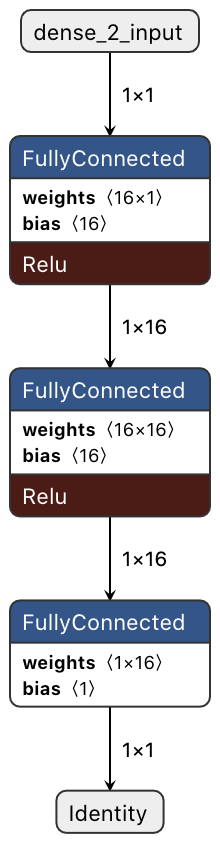
\includegraphics[width=0.6\textwidth]{figures/hello_world_graph.png}
         \caption{Hello World}
         \label{fig:netron_hello_world}
     \end{subfigure}
     \hfill
     \begin{subfigure}[b]{0.3\textwidth}
         \centering
         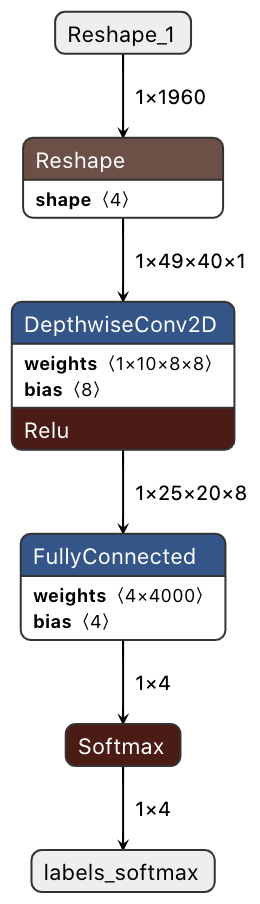
\includegraphics[width=0.8\textwidth]{figures/micro_speech_graph.png}
         \caption{Micro Speech}
         \label{fig:netron_mirco_speech}
     \end{subfigure}
     \hfill
     \begin{subfigure}[b]{0.3\textwidth}
         \centering
         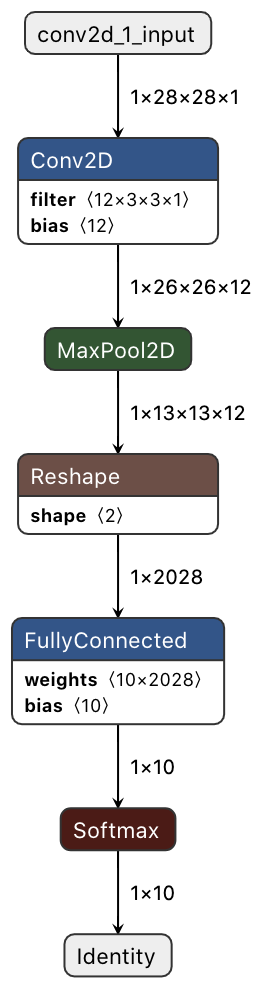
\includegraphics[width=0.8\textwidth]{figures/mnist_graph.png}
         \caption{MNIST}
         \label{fig:netron_mnist}
     \end{subfigure}
        \caption{TFLite Model Graphs per Example}
        \label{fig:netron}
\end{figure}

\section{Implementation}

\subsection{Hello World}

Most of the Hello World Demo was running out of the box after the toolchain was updated to be compatible with the latest tensor flow version.

Shortly the first example was running an initial version of a custom benchmarking module was added to the source code which allows to extract execution times of several parts of the main program loop.

\subsection{Micro Speech}

The hardest challenge of the Micro Speech example was streaming the input samples for the network in real-time which requires a sufficient execution speed of the four main processes:

\begin{itemize}
    \item \textbf{Feature Generation:} Uses quite large ring-buffers to fit multiple time slots. If the main loop takes to long for one iteration, the buffer size has to be increased to prevent an overflow. Spectrogram-slices are generated with the new samples.
    \item \textbf{Invoke Network:} A set of spectrogram slices is feed into the the network input. The quantized output is an array of signed chars representing a probability of the four classes \lstinline{yes,no,unknown,silence}
    \item \textbf{Post processing Results:} To reduce false positives and handle fluctuations a moving average has to be applied to the history of network outputs. Combined with thresholds and other parameters the detected class of command with the respective probability is returned 
    \item \textbf{Command Responding:} If there is a new command detected, the result is displayed on the screen and/or printed on the serial terminal. 
\end{itemize}

After the microphone functionality was added and the buffer size tuned the model was not responsive at all. It was unclear if the reason for this issue was a to slow processor but at this point the development was shifted to the faster F7 Board. In the meantime, by enabling the support of CMSIS-NN the execution time of the Invoke step was drastically reduced resulting in a higher sample throughput. 

The final step which was required to achieve meaningful results with the application was reducing thresholds and tuning timing constants an the post processing step. In fact, this lead to more wrong detections but at least allowed to detect some correct samples in the end.

To find out if the rather bad performance of the network was cause by the microphone samples being too different compared to the original data set much time was invested adding the ability to provide samples from WAV-files via the on-board SD-card slot. As the manufacturer libraries for the audio codecs did not support playing mono audio. The original 1 second WAV files had to be converted to stereo files beforehand with a custom script.

\subsection{MNIST}

The well-known MNIST dataset contains ten thousands of hand written digits. They have a quite small resolution and only feature grayscale values to reduce the size and therefore the complexity of the samples.

To use feed digits written via a touchscreen into the network some prepossessing is needed:

\begin{itemize}
    \item Find a suitable brush size (circle radius) for the input
    \item Interpolate between inputs to get a smoother line
    \item Downscale the input image to 28x28 pixels with  a proper filter
    \item Convert the color space of the display to 8 bpp grayscale
    \item Invert the color spectrum (whit on black instead of black on white)
\end{itemize}

Similar to the MNIST implementation SD-Card support for feeding original samples instead of touchscreen data was also added. Scripts to generate board-compatible BMP files are provides with the source code. 

While some of the predictions have been very accurate the network as not capable some digits neither with original samples nor with touchscreen inputs. This leads to the conclusion that the model architecture needs some further tuning.

As the TFLite Micro currently does not support unsigned 8 bit quantization the training script had to be modified to use signed values between -128 and 127. This fact also had to be considered when preparing the input tensor for the network.

Figure \ref{fig:gifs} shows the examples in running on the actual hardware. Animated versions of these graphics can be found in the respective repository!

\begin{figure}[h]
     \centering
     \begin{subfigure}[b]{0.3\textwidth}
         \centering
         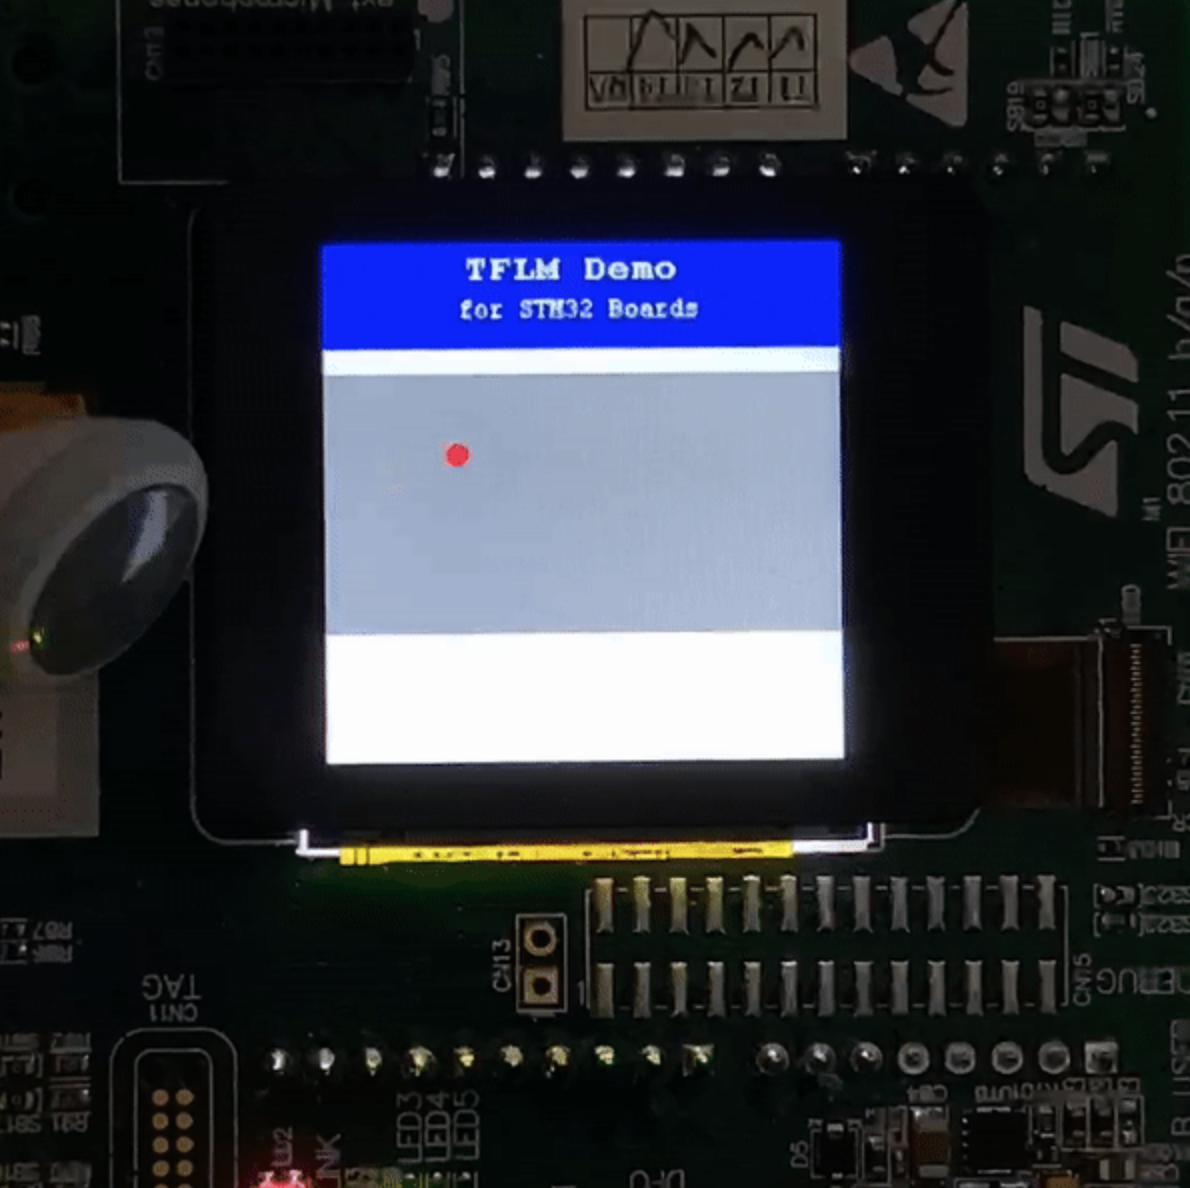
\includegraphics[width=0.8\textwidth]{figures/hello_world_gif.png}
         \caption{Hello World}
         \label{fig:gif_hello_world}
     \end{subfigure}
     \hfill
     \begin{subfigure}[b]{0.3\textwidth}
         \centering
         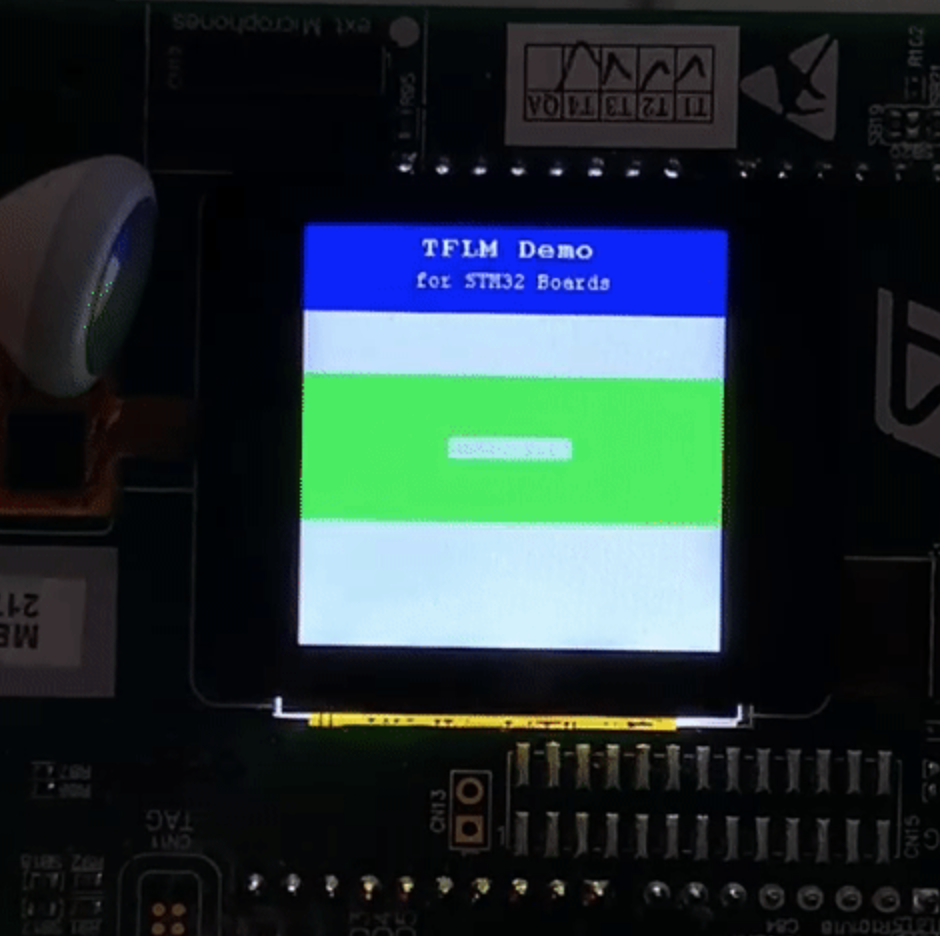
\includegraphics[width=0.8\textwidth]{figures/micro_speech_gif.png}
         \caption{Micro Speech}
         \label{fig:gif_mirco_speech}
     \end{subfigure}
     \hfill
     \begin{subfigure}[b]{0.3\textwidth}
         \centering
         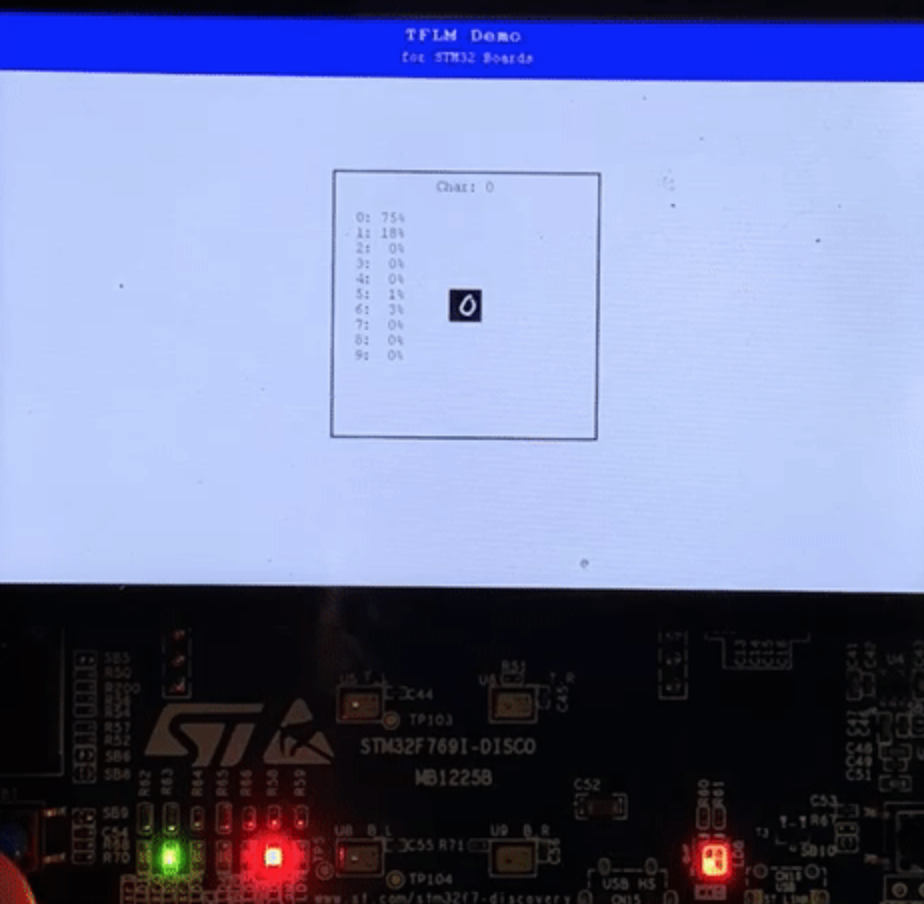
\includegraphics[width=0.8\textwidth]{figures/mnist_gif.png}
         \caption{MNIST}
         \label{fig:gif_mnist}
     \end{subfigure}
        \caption{Examples running on the STM32 Boards}
        \label{fig:gifs}
\end{figure}

\section{Documentation}

To make the code easier to maintain, the common toolchain parts have been outsourced to submodules. A wrapper repository was added to provide links to all actual examples and to provide overarching documentation. This reduced the amount of redundant documentation by only providing example specific explanations together with the submodules. The resulting project structure is easy extendable and can be found on GitHub\footnote{\url{https://github.com/PhilippvK/stm32-tflm-demos}}.

\chapter{Evaluation}



\section{Board Metrics}

Before reviewing the collected metrics of the models running on the hardware platform, the main properties of both evaluation boards are shown in the following table. Its not hard to tell that the F7 board features a much faster MCU than the F4 counterpart while both of them are quite good in terms of available memory resources.

\begin{table}[h]
\begin{tabular}{|l|c|c|l|}
\hline
& \multicolumn{2}{c|}{\textbf{Boards}} &\\\hline
\textbf{Metrics} & STM32F413HDISCOVERY & STM32F769IDISCOVERY & \textbf{Units} \\\hline
Clock Frequency   & 100  & 216    & \textit{MHz}         \\
Special Features  & -        & Double Issue, I/D-Cache      & \textit{-}       \\
Flash Memory      & 1.5      & 2      & \textit{MB}          \\
SRAM Memory       & 256                              & 512                              & \textit{kB}    \\\hline
\end{tabular}
\end{table}

\section{Memory Usage}

See the following table for approximate Flash and RAM usage

\begin{table}[h]
\begin{tabular}{|l|c|c|c|l|}
\hline
& \multicolumn{3}{c|}{\textbf{Examples}} &\\\hline
\textbf{Type}                        & hello\_world & mirco\_speech & mnist & \textbf{Units} \\\hline
Model Size (FLASH)                      & 2              & 18              & 23      & \textit{kB}     \\
TensorArena Size (SRAM) & 1              & 7               & 11      & \textit{kB}\\\hline  
\end{tabular}
\end{table}

According to a paper\cite{banbury2020micronets}, the approximated Memory requirements for TFLite Micro are the following:

\begin{itemize}
    \item SRAM: ~4 kB
    \item FLASH: ~37 kB
\end{itemize}

\section{Number of Ops}

The FLOPS (not FLOP/s) of the model graph should give an idea on how many additions and multiplications are needed for a single invocation on the network. The stated values are highly approximatively as they do not take every TF operation into account and are generated before quantization on the eras models itself.

\begin{table}[h]
\begin{tabular}{|c|c|c|}
\hline
\multicolumn{3}{|c|}{\textbf{Examples}}\\\hline
hello\_world & mirco\_speech & mnist        \\\hline
41 \textit{FLOPS}     & 689980 \textit{FLOPS}  & 202810 \textit{FLOPS}\\\hline
\end{tabular}
\end{table}

\section{Runtime Measurements}

The time spend in different sections on the main program \lstinline{loop()} is analyzed quantitatively in the following section. The results are heavily influenced by the implementation of the network, as interrupts, serial communication and I/O-activity may be present during the measurements. Therefore and because of the reasons mentioned above, the relationship between the FLOPS and the invocation time is not linear.

All values have been collected by averaging over ~1 minute of runtime with the CMSIS-NN kernels enabled.

The program loop was splitted in the following intervals for all 3 examples: \lstinline{POPULATE/INVOKE/RESPOND}

\begin{table}[h!]
\begin{tabular}{|l|l|c|c|c|l|}
\hline
& &\multicolumn{3}{c|}{\textbf{Examples}} &\\\hline
\textbf{Section} & \textbf{CPU} & hello\_world  & mirco\_speech & mnist                                         & \textbf{Units} \\\hline
\multirow{2}{*}{Populate}     &  F4              & $\sim$0 & 38 & 132 & \multirow{2}{*}{\textit{ms}} \\
&F7&$\sim$0&11&88&\\\hline
\multirow{2}{*}{Invoke}     &  F4              & $\sim$0 & 49 & 34 & \multirow{2}{*}{\textit{ms}} \\
&F7&$\sim$0&52&13&\\\hline
\multirow{2}{*}{Respond}     &  F4              & $\sim$0 & $\sim$0 & 125 & \multirow{2}{*}{\textit{ms}} \\
&F7&$\sim$0&$\sim$0&93&\\\hline
\end{tabular}
\end{table}

\section{CMSIS-NN Optimizations}

In the following, the differences in execution time for running the model with the cmsis-nn kernels turned ON/OFF are compared briefly. The extend of the improvement depends on the used operations in the graph because only the following kernels are currently supported:

\begin{multicols}{2}
\begin{itemize}
    \item \lstinline{add}
    \item \lstinline{conv}
    \item \lstinline{depthwise_conv}
    \item \lstinline{fully_connected}
    \item \lstinline{mul}
    \item \lstinline{pooling}
    \item \lstinline{softmax}
    \item \lstinline{svdf}
\end{itemize}
\end{multicols}

\textit{Notice:} The values for the STM32F413HDISCOVERY are omitted here as they relatively similar compared to the F7 values.

\begin{table}[h]
\begin{tabular}{|l|l|l|l|l|l|}
\hline
\multicolumn{2}{|l|}{} & \multicolumn{3}{c|}{\textbf{Examples}} &\\\hline
\multicolumn{2}{|l|}{\textbf{Settings}}  & hello\_world & mirco\_speech & mnist & \textbf{Units} \\\hline
\multirow{2}{*}{CMSIS\_NN} & OFF              & $\sim$1                 & 413\footnote{The model is unusable without the CMSIS-NN optimized kernels as the program loop does not run often enough to keep up with the incoming audio stream.}                 & 52               & \textit{ms}             \\
 & ON               & $\sim$0                 & 52                       & 13               & \textit{ms}              \\\hline
\multicolumn{2}{|l|}{Difference}                   & (?)                     & (-87)                    & (-75)            & \textit{\%}           \\\hline  
\end{tabular}
\end{table}

\section{Details on Results}

The previously presented results can also be found in the repos documentation alongside with a short manual on how to obtain those numbers. See: \url{https://github.com/PhilippvK/stm32-tflm-demos/blob/main/docs/Metrics.md}

\chapter{Conclusions}

\section{Summary}

While the goal of the research internship was to implement two of the examples from the TinyML book on real hardware, it was possible to get the MNIST example (which is not covered in the book) running as well. In terms of model performance, further work is required but the current implementation suffices as a demonstration to show the capabilities of TinyML on respective microcontroller platforms. As the work on this topic is definitely not done, a short outlook is presented in the following section.

\section{Outlook}

Here is a list of task or extensions which could improve the project even more in the future:

\begin{itemize}
    \item Support USB-Storage as alternative to SD-Card
    \item Add TinyFace Model\cite{teodorfratiloiu2020}
    \item Merge Deployment and Evaluation Flow with EDA RISCV-toolchain
    \item Enable usage of FreeRTOS instead of baremetal
    \item Add possibility to parse results via UART
    \item Feed samples via UART for automated testing\\[2em]
    $\Rightarrow$ Extract data on the accuracy of the models
\end{itemize}

\backmatter

\bibliographystyle{IEEEtran}
\bibliography{literature}

\end{document}
